\documentclass[a4paper,twocolumn,12 pt]{article}
\usepackage{silence}  % pacchetto che permette di sopprimere warnings cagacazzo
\WarningFilter{latex}{`h' float specifier changed to `ht'}
\usepackage{geometry}
 \geometry{
 a4paper,
 total={170mm,257mm},
 left=20mm,
 top=20mm,
 }
\usepackage[T1]{fontenc}
\usepackage[utf8]{inputenc}
\usepackage[english,italian]{babel}
\usepackage{url}
\usepackage{graphicx}
\usepackage{amsmath}
\usepackage{amstext}
\usepackage{booktabs}
\usepackage{wrapfig}
\usepackage{siunitx}
\usepackage{subcaption}
\usepackage{amssymb}
\usepackage{animate}
\usepackage{csquotes}
\usepackage{biblatex}
\usepackage{xurl}   % compatta gli url
\usepackage{hyperref}
\usepackage{indentfirst}
\usepackage[font=footnotesize, labelfont=bf]{caption}
% \usepackage[LGRgreek]{mathastext}
\usepackage{esint}
\makeatletter
% make esint definition in line with amsmath
\@for\next:={int,iint,iiint,iiiint,dotsint,oint,oiint,sqint,sqiint,
  ointctrclockwise,ointclockwise,varointclockwise,varointctrclockwise,
  fint,varoiint,landupint,landdownint}\do{%
    \expandafter\edef\csname\next\endcsname{%
      \noexpand\DOTSI
      \expandafter\noexpand\csname\next op\endcsname
      \noexpand\ilimits@
    }%
  }
\makeatother
\usepackage{multirow}
\usepackage{multicol}
\usepackage{float}
\usepackage{subdepth}

\addbibresource{citations.bib}
\hbadness=1000000

\pagestyle{plain}

\title{\textbf{Stima della concentrazione parziale di siti sostituzionali in polveri di perovskite doppia}}
\author{\textbf{Luca Sanna, 60/68/65275}}
\date{\textbf{06/12/2025}}


\begin{document}
\twocolumn[
\maketitle
  \begin{@twocolumnfalse}\maketitle
        \begin{abstract}\noindent
          L'obiettivo dell'esperienza di laboratorio è calcolare la concentrazione parziale $x$ di Ag e Na, come siti sostituzionali in polveri di perovskite doppia del tipo Cs$_2$Ag$_{1-x}$Na$_x$InCl$_6$. Tramite analisi Rietveld, si sono ottenuti i risultati per due diversi campioni di $(0.180 \pm 0.006) \%$ e $(0.560 \pm 0.011) \%$, di discrepanza con i valori nominali rispettivamente $7.31\%$ e $4.92\%$.
        \end{abstract}
  \end{@twocolumnfalse}
]

\raggedbottom
\section*{Introduzione}
La tecnica XRD (X-Ray Diffraction) permette di sondare il reticolo reciproco di un sistema cristallino.

\begin{figure}[htbp]
  \centering
  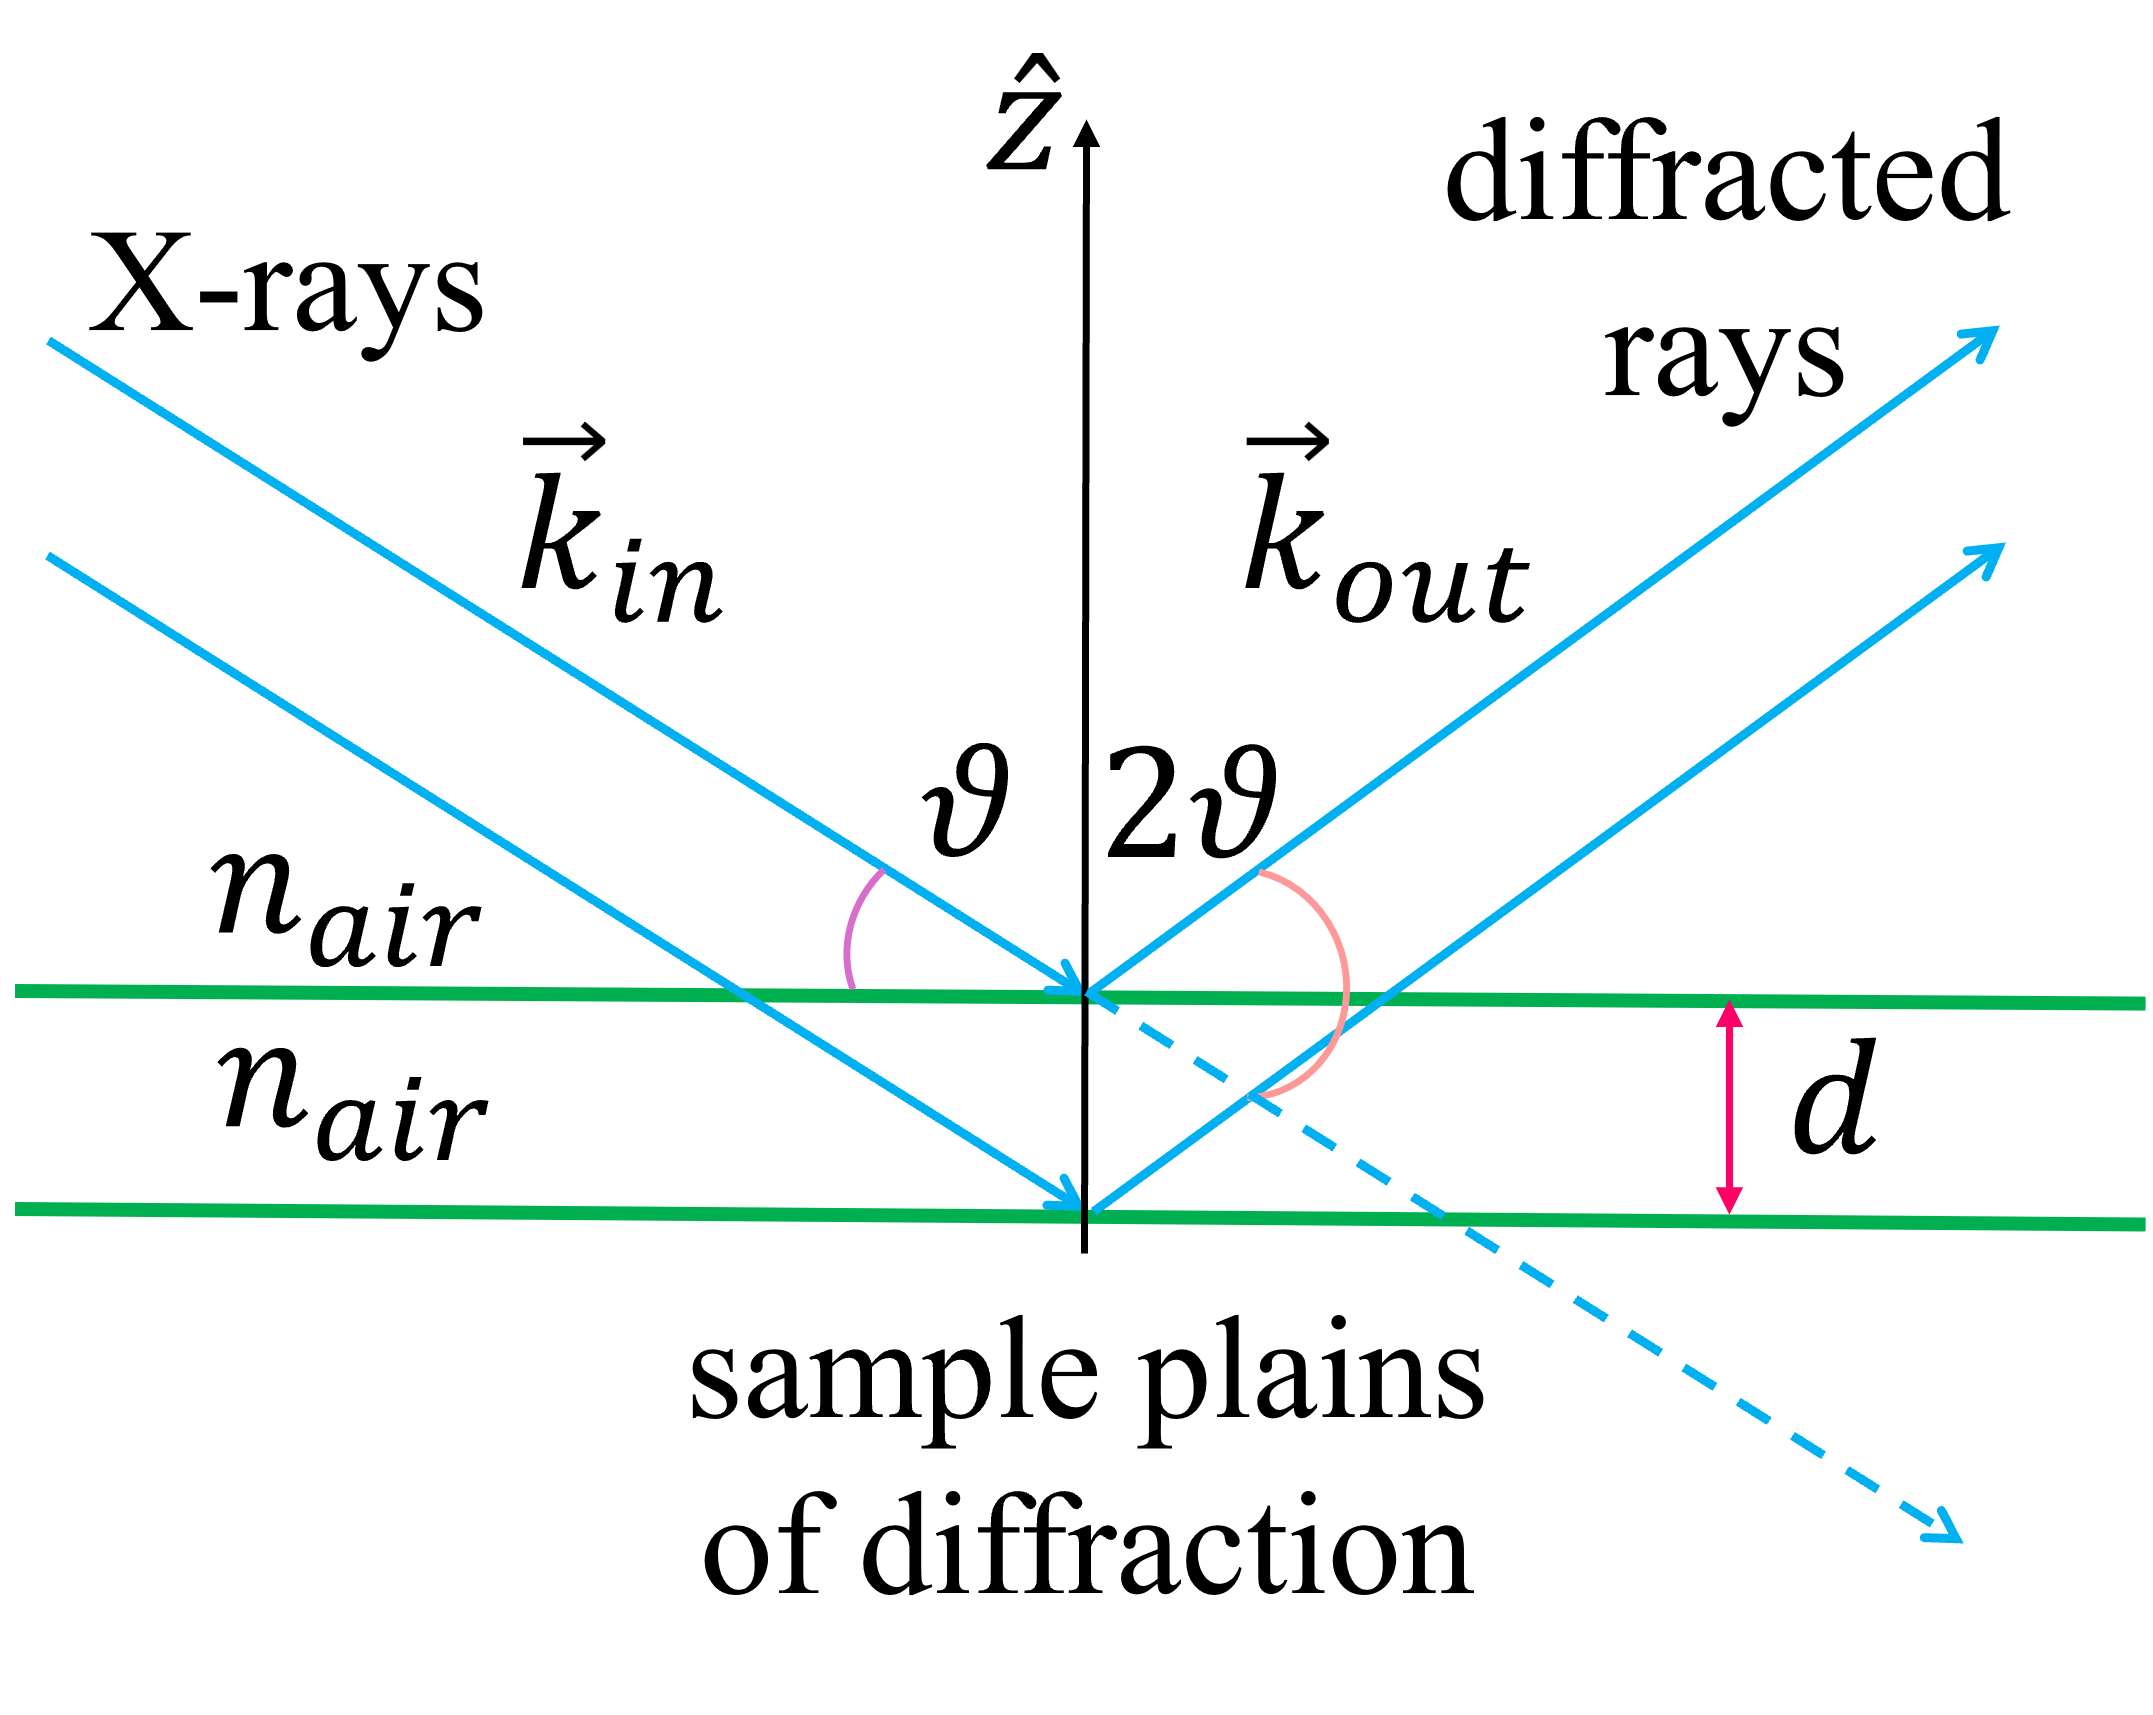
\includegraphics[width = 0.8\linewidth]{../Bragg.png}
  \caption{Schema esemplificativo della legge di Bragg.}
  \label{fig: Bragg}
\end{figure}

Radiazione elettromagnetica X, di lunghezza d'onda $\lambda$ comparabile con le tipiche distanze inter-atomiche in un cristallo, e di vettore d'onda $\vec{k}_{in}$, è diffratta costruttivamente, con vettore d'onda $\vec{k}_{out}$, secondo la \emph{legge di Bragg}:
\begin{equation}
  nd \sin \vartheta = m \lambda,
  \label{eq: Bragg}
\end{equation}
dove $n$ è l'indice di rifrazione del mezzo (solitamente aria, $n = 1$), $d$ è la distanza tra i piani cristallini che rispettano la stessa orientazione, $\vartheta$ è l'angolo di incidenza rispetto alla direzione parallela al piano di diffrazione, $m$ è l'ordine diffrattivo (si consideri soltanto il primo ordine, $m = 1$). La figura \ref{fig: Bragg} permette di visualizzare il fenomeno sopra descritto.

Il risultato della misura è un \emph{diffrattogramma}, ovvero la distribuzione dei conteggi relativi ai fotoni diffratti con successo sullo schermo di acquisizione, in funzione dell'angolo diffrattivo $2 \vartheta$. A ogni orientazione privilegiata dei piani cristallini corrisponde un picco nel grafico. Maggiore il grado di simmetria della struttura reticolare, minore il numero di picchi; più numerosa la famiglia di piani osservata, maggiore l'intensità del picco associato.

Nel contesto del lavoro di laboratorio proposto, è rilevante il concetto di \emph{polvere}. Si definisce una polvere ideale un campione costituito da un'infinito numero di cristalliti (reticoli cristallini che mantengono la stessa struttura e orientazione) e caratterizzato da un'infinito numero di orientazioni casuali. Il diffrattogramma tipico di una polvere è dunque costituito di numerosi picchi specifici di quel determinato materiale, e rappresentano un'\emph{impronta digitale} che ne permette l'identificazione.

Il fit di un diffrattogramma permette di ottenere informazioni qualitative e quantitative sul materiale osservato. Di rilievo per l'esperimento in questione, sono la costante reticolare $a$ e l'occupazione, totale e/o parziale $x$, di un certo elemento nella cella unitaria della struttura cristallina. Si consideri l'esempio delle perovskiti doppie, che rispettano la formula chimica ridotta più generale ABX$_3$; l'elemento contrassagnato dalla lettera B può essere sostituito da due o più elementi diversi, (nel caso più semplice di due, essi siano C e D) che condividono l'occupazione totale sui siti originali. La formula chimica diventa così AC$_{1-x}$D$_x$X$_3$, che identifica un cristallo di costante reticolare $a_{\text{C}_{1-x}\text{D}_x}$. Considerando le costanti reticolari $a_{\text{C}}$ e $a_{\text{D}}$ delle perovskiti rispettivamente ACX$_3$ e ADX$_3$, si enuncia la \emph{legge di Vegard}:
\begin{equation}
  a_{\text{C}_{1-x}\text{D}_x} = (1-x)a_{\text{C}} + xa_{\text{D}}.
  \label{eq: Vegard}
\end{equation}
L'equazione \ref{eq: Vegard}, che ha origine euristica, è un'approssimazione che si basa sull'assunzione che la temperatura sia la stessa per entrambi i composti ACX$_3$ e ADX$_3$ e che essi siano in forma pura prima che la miscela dia origine alla sostanza risultante AC$_{1-x}$D$_x$X$_3$.


\section*{Esperimento}
Uno strumento XRD può effettuare misure secondo diverse geometrie, in funzione del tipo di campione e del genere di misura che si vuole ottenere.

\begin{figure}[htbp]
  \centering
  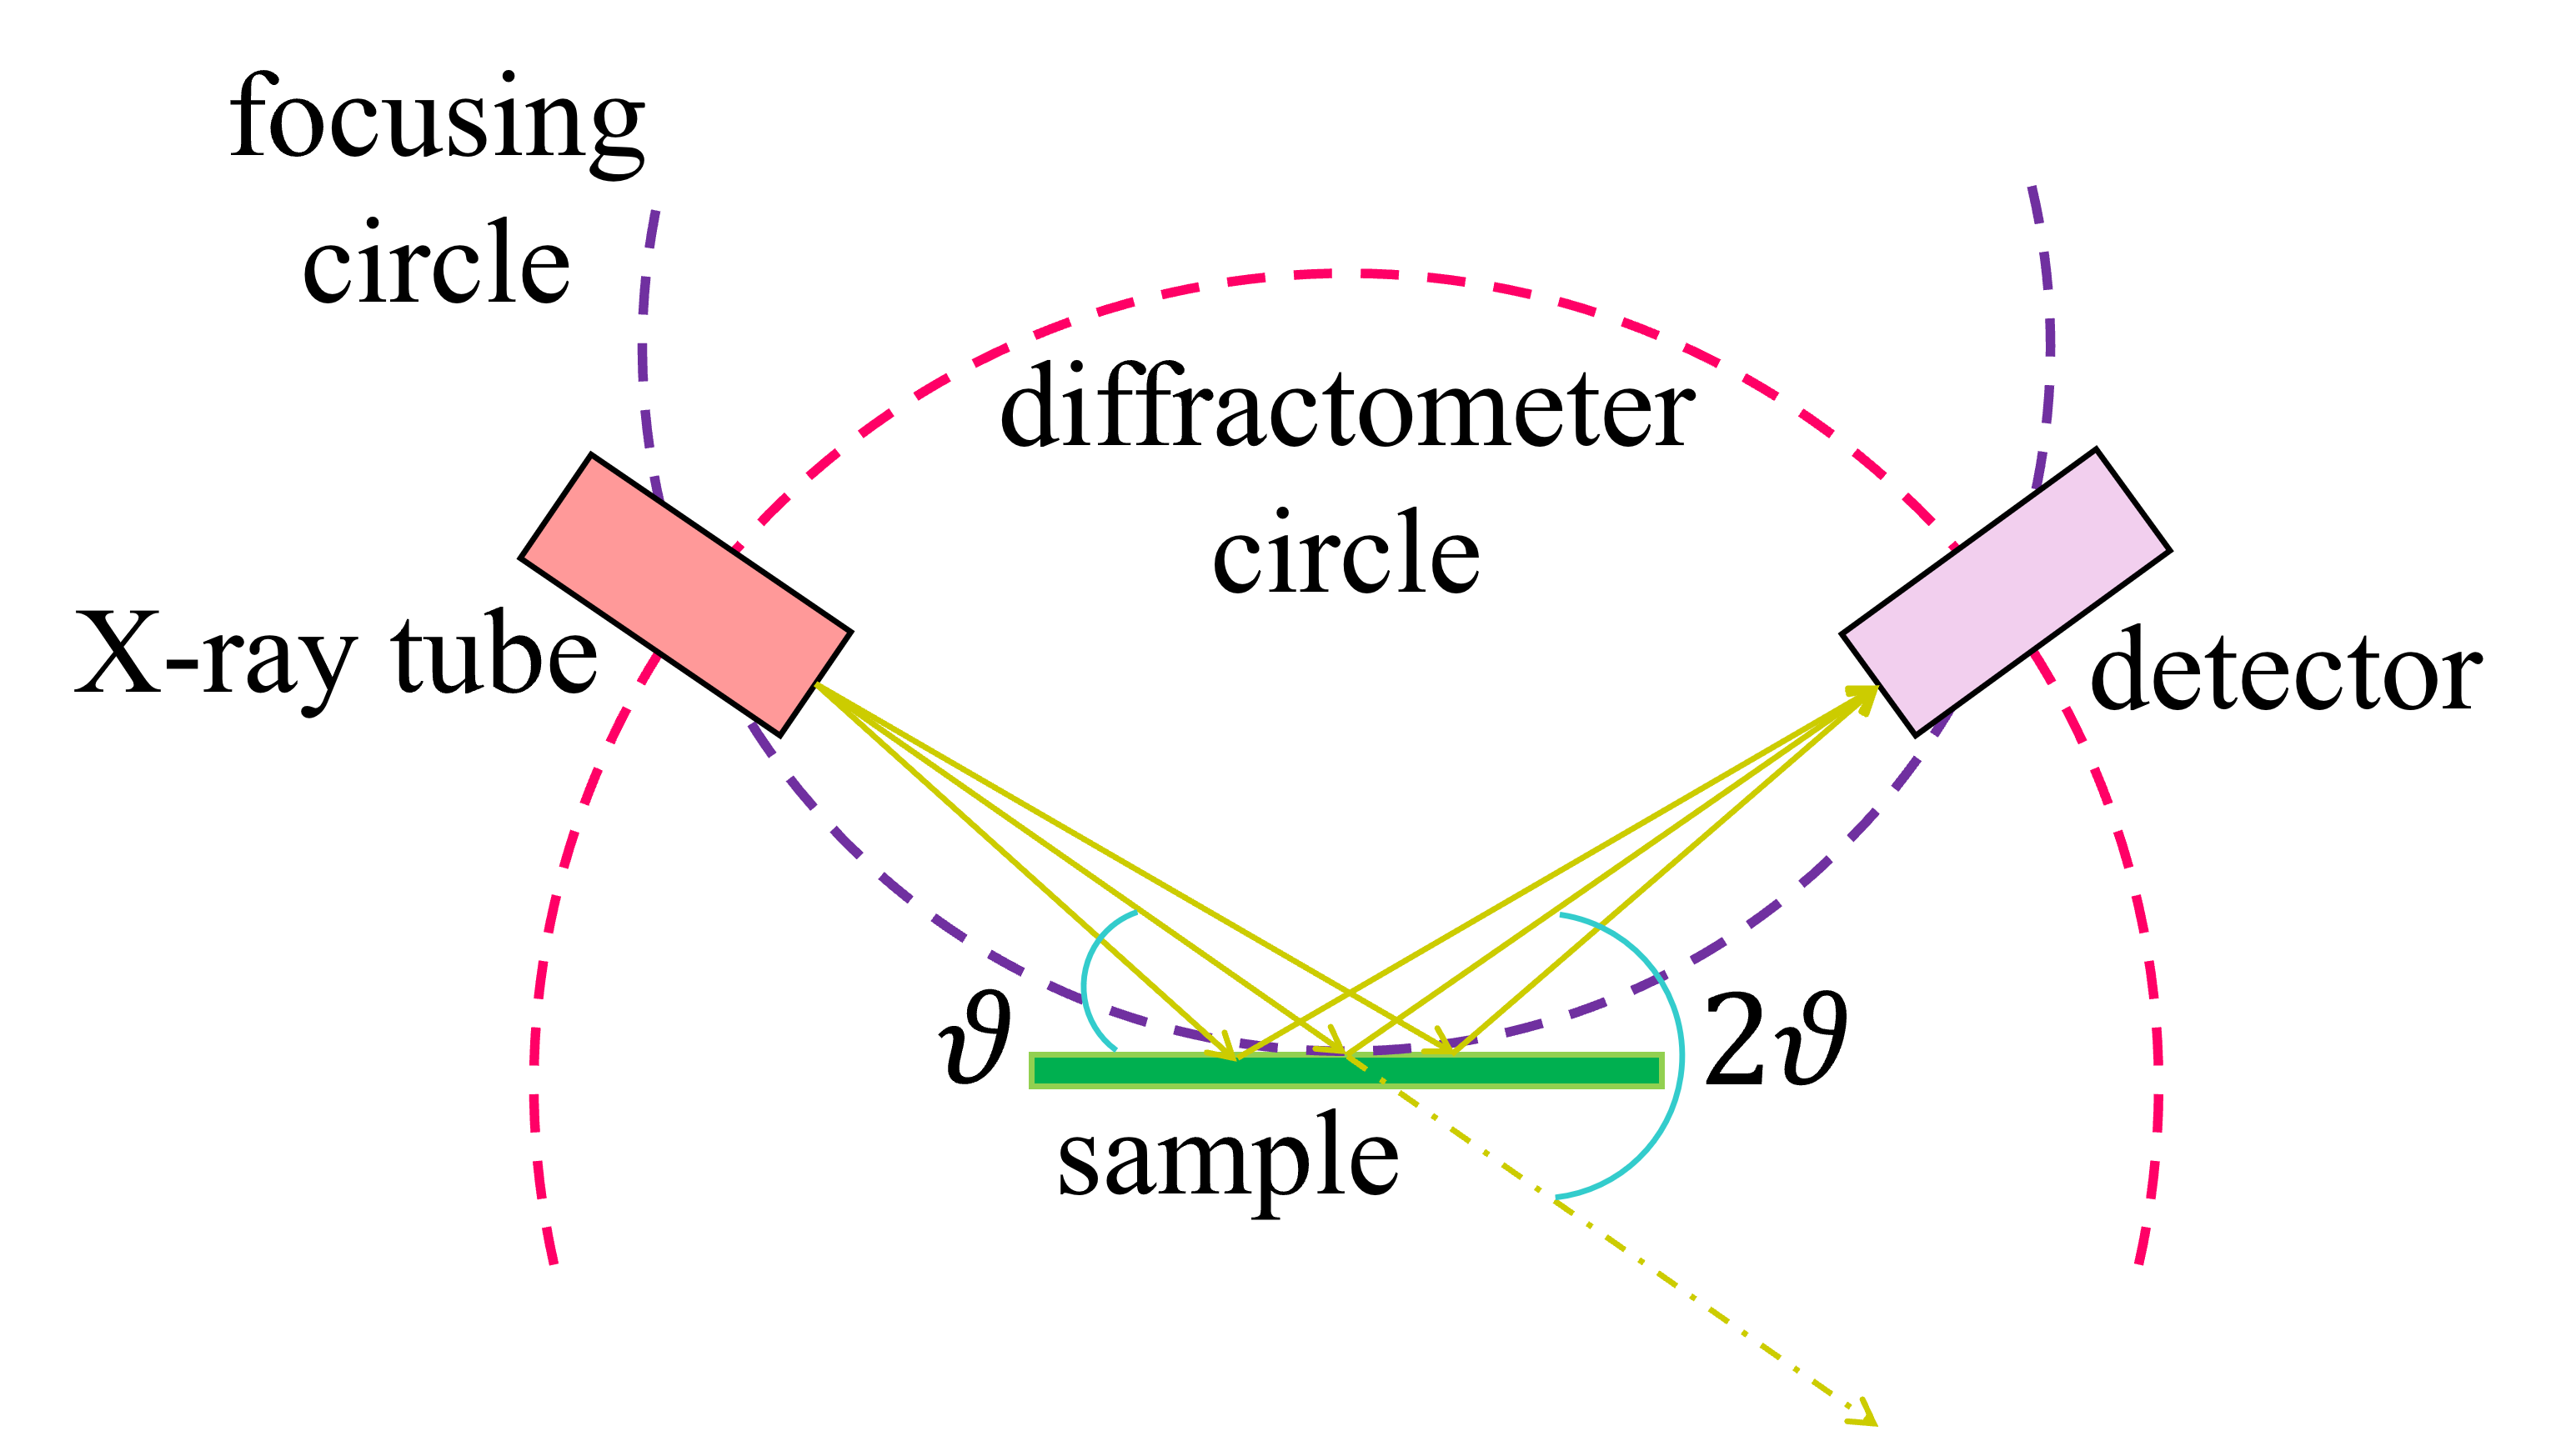
\includegraphics[width = 1\linewidth]{../Bragg-Brentano.png}
  \caption{Schema della geometria XRD Bragg-Brentano.}
  \label{fig: Bragg-Brentano}
\end{figure}

La geometria Bragg-Brentano, rappresentata essenzialmente in figura \ref{fig: Bragg-Brentano}, è utilizzata proprio nel caso di misure XRD su polveri. Il genere di scansione è $\vartheta / 2\vartheta$, ovvero il tubo a raggi X e il rilevatore si muovono simultaneamente lungo una circonferenza di raggio fissato, mantenendo costante il rapporto $\vartheta / 2\vartheta$. La sorgente diverge sul campione, e si rifrange sul rilevatore grazie a lenti convergenti. L'angolo di incidenza $\vartheta$ determina il raggio della circonferenza di fuoco, ovvero quali punti sulla superficie del campione possono essere catturati, con la migliore precisione disponibile, dal rilevatore. Questo percorso fittizio costituisce un limite alla qualità della misura; infatti, la superficie del campione è ideale sia tangente alla circonferenza e il punto di tangenza deve trovarsi sul luogo della superficie che si desidera studiare. L'effetto di un posizionamento non ottimale risulta nello spostamento e/o allargamento dei picchi.

Nello specifico dello strumento adoperato~\supercite{XRD:spec}, il goniometro che individua la circonferenza di diffrazione è perpendicolare alla superficie del campione e il tubo a raggi X possiede un anodo in rame. L'importanza del materiale, sorgente per i fotoni incidenti, risiede nella lunghezza d'onda caratteristica di emissione; elementi diversi provocano una traslazione complessiva del diffrattogramma, che ostacola un confronto diretto tra grafici ottenuti con tubi a raggi X di anodo costituito da materiale differente.

Le polveri osservate sono quattro perovskiti, di cui due ternarie, Cs$_2$AgInCl$_6$ e Cs$_2$NaInCl$_6$, e due quaternarie, nominalmente Cs$_2$Ag$_{0.8}$Na$_{0.2}$InCl$_6$ e Cs$_2$Ag$_{0.4}$Na$_{0.6}$InCl$_6$, miscele parziali delle prime. Al fine di ottenere una condizione quanto più vicina a quella di polvere ideale, si rende necessario fare uso di mortaio e pestello in agata.


\section*{Risultati}
Il fit di ogni diffrattogramma è stato realizzato mediante il software MAUD~\supercite{maud}, che permette di usufruire del \emph{raffinamento Rietveld}; si tratta di un criterio di regressione che si basa sul \emph{metodo dei minimi quadrati non-lineare}. L'obiettivo è minimizzare la \emph{Weighted Sum of Sqaures}:
\begin{equation}
  WSS = \displaystyle\sum_{k} w_k \left\lbrack I^{(exp)}_k - I^{(fit)}_k \right\rbrack^2,
  \label{eq: WSS}
\end{equation}
dove $k$ è un indice che corre su ogni $k$-esima misura del diffrattogramma, $I^{(exp)}_k$ e $I^{(fit)}_k$ sono rispettivamente l'intensità attesa e quella calcolata tramite il fit, e
\begin{equation}
  w_k = \frac{1}{\sqrt{I^{(exp)}_k}}
  \label{eq: pesi}
\end{equation}
è il peso $k$-esimo che la $k$-esima misura di intensità attesa porta nell'ottimizzazione dell'equazione \ref{eq: WSS}.

\begin{figure}[htbp]
  \centering
  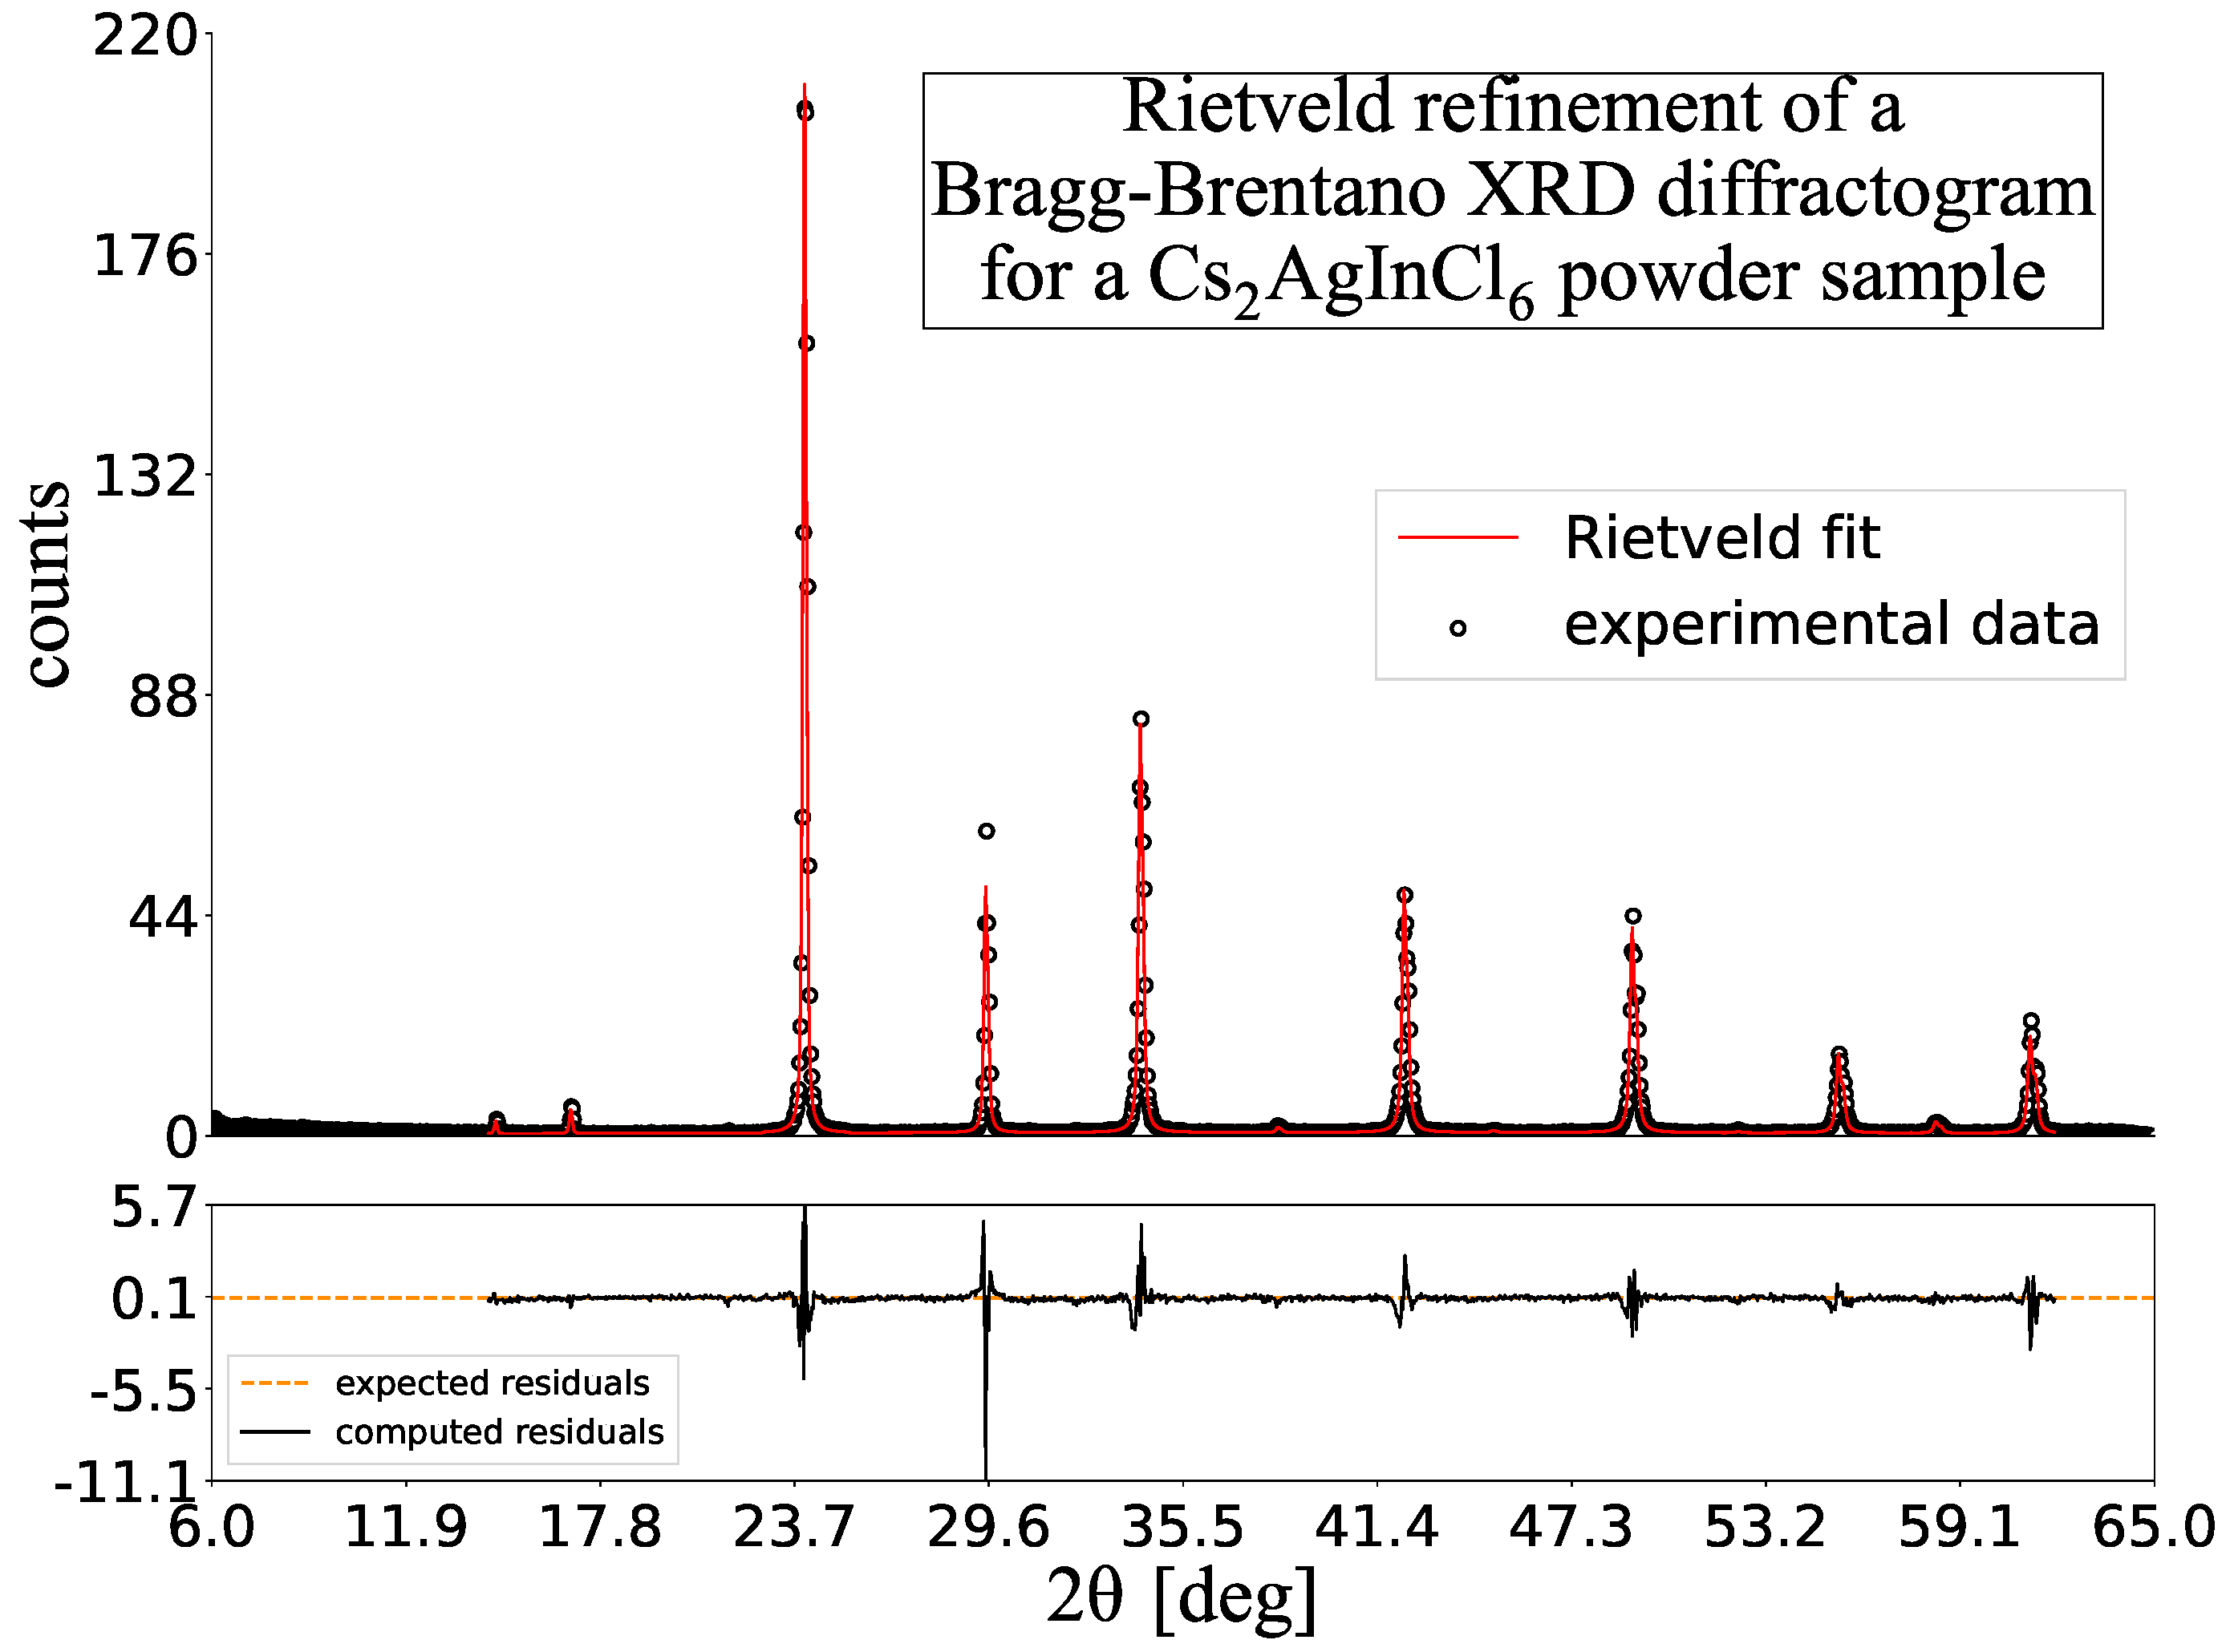
\includegraphics[width = 1\linewidth]{../Datasets/A01_Cs2AgInCl6.pdf}
  \caption{Fit Rietveld per un diffrattogramma di Cs$_2$AgInCl$_6$ in polvere.}
  \label{fig: Ag}
\end{figure}
\begin{figure}[htbp]
  \centering
  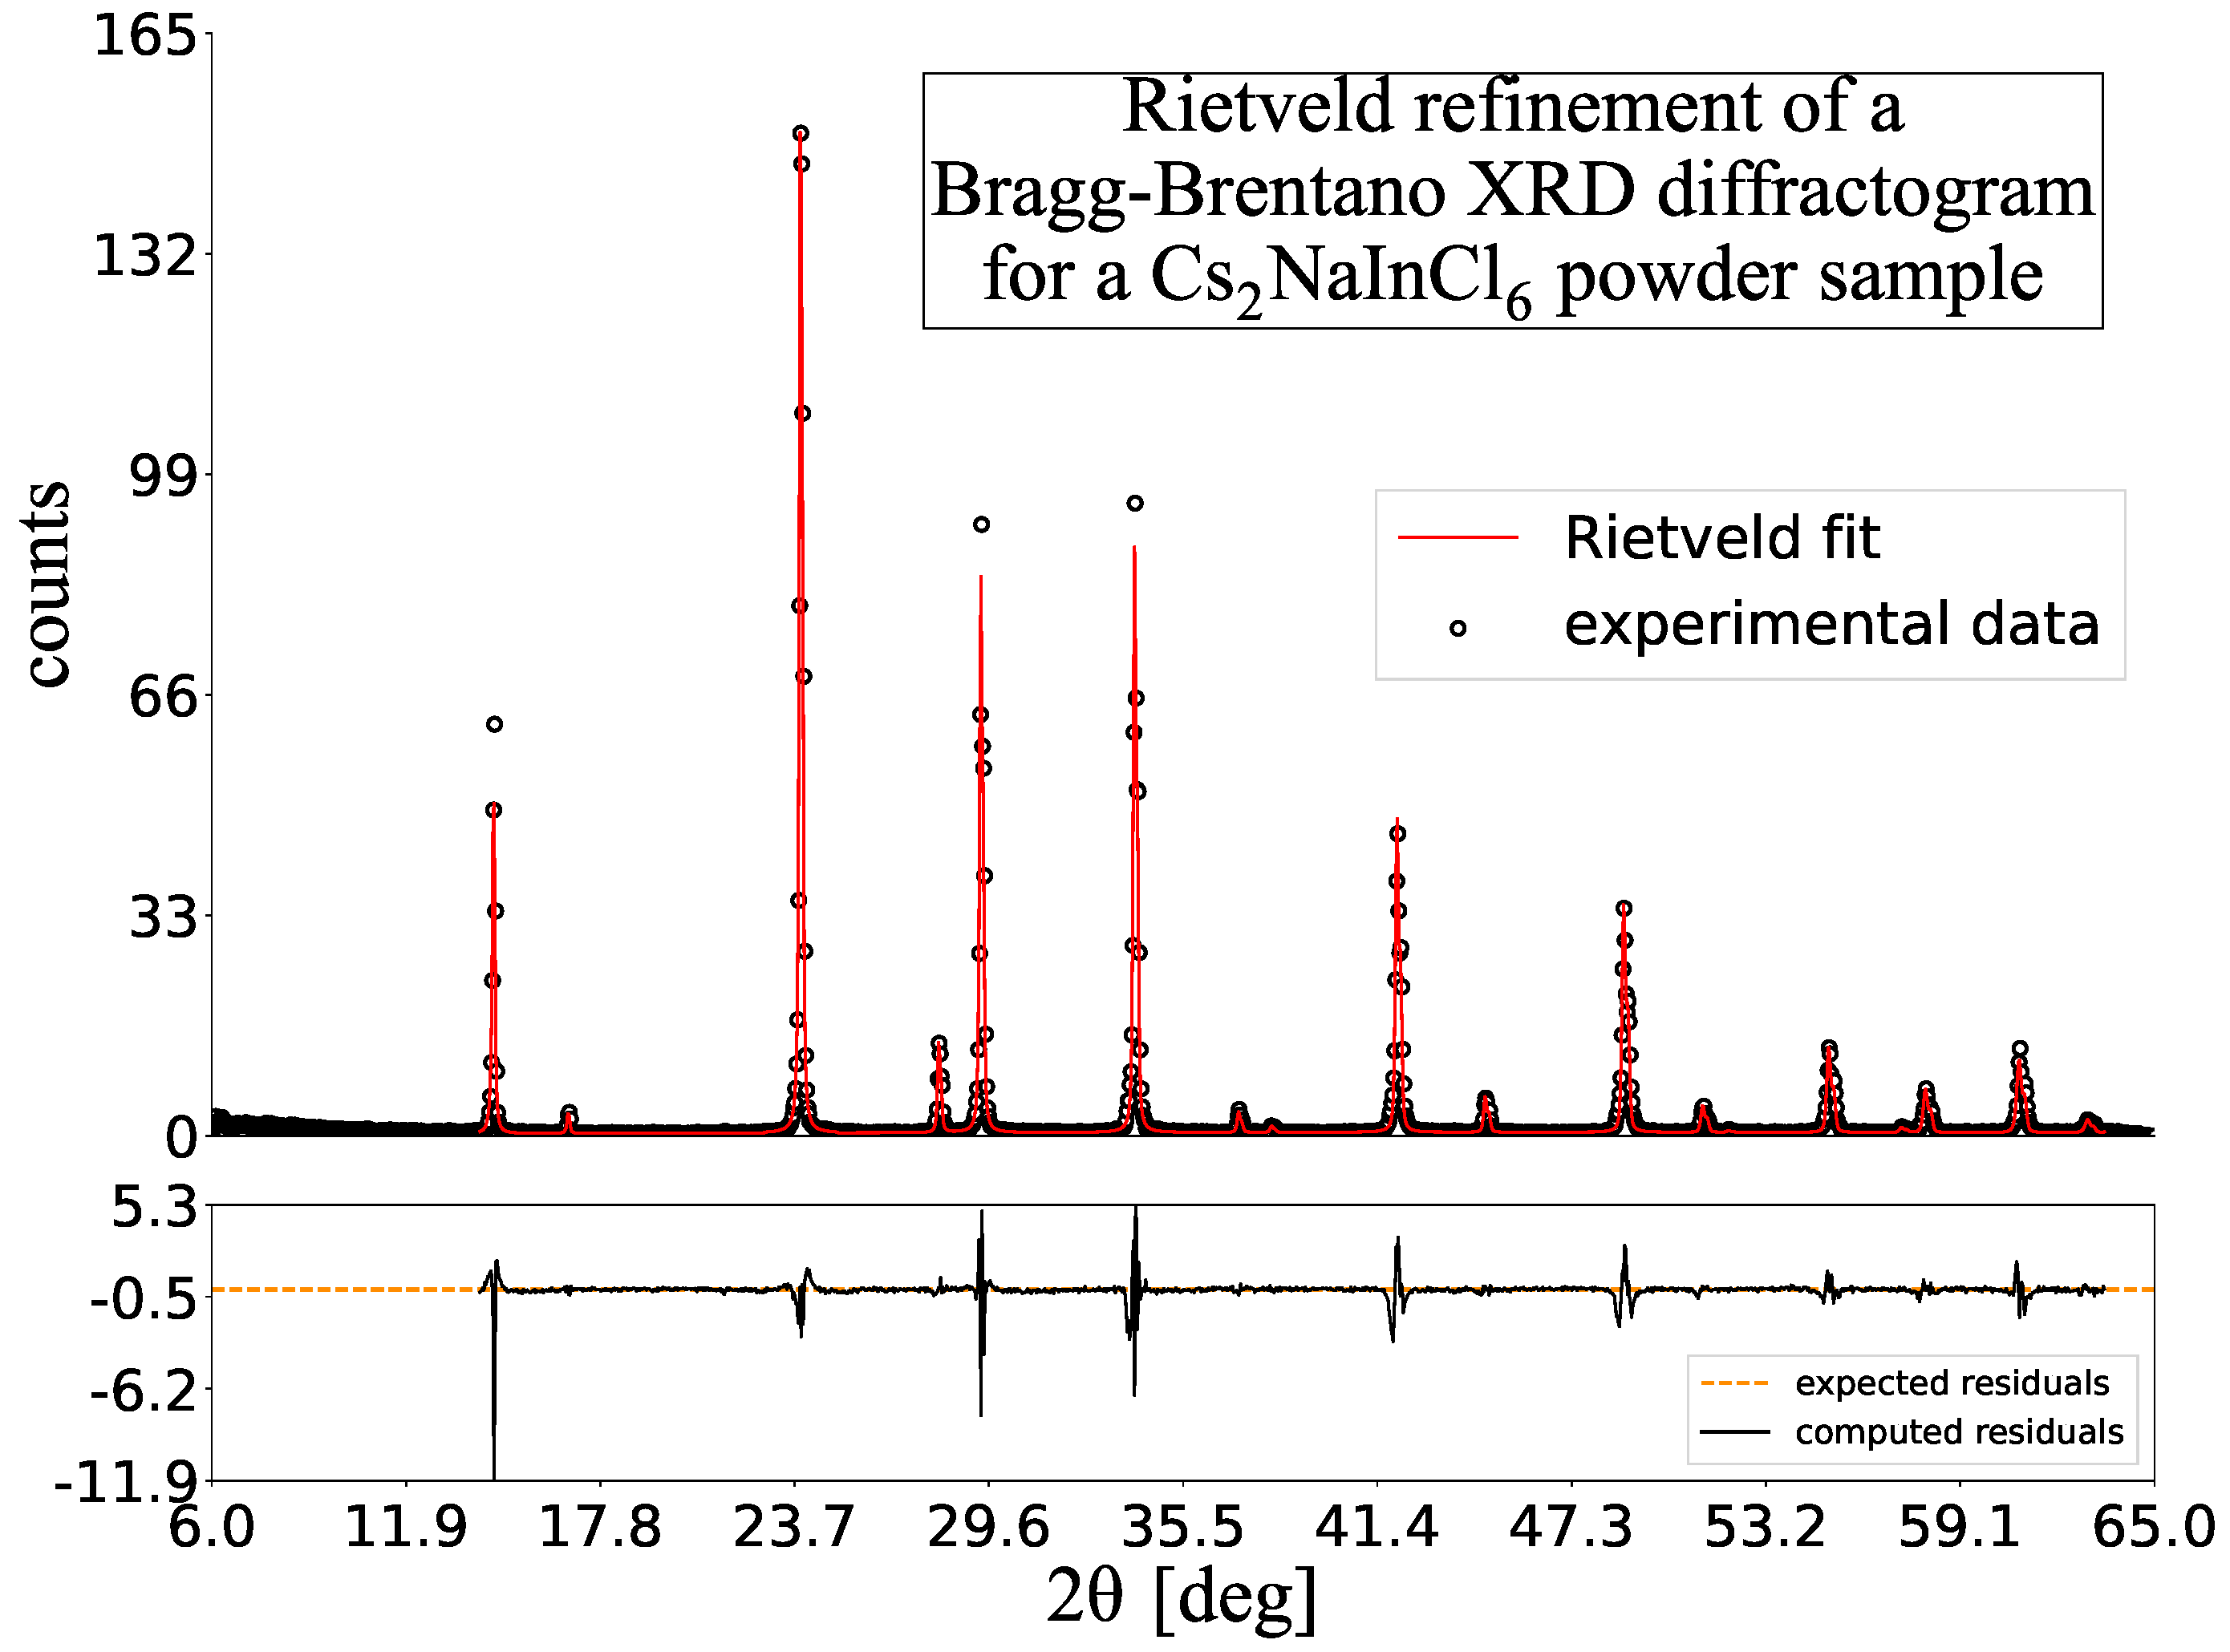
\includegraphics[width = 1\linewidth]{../Datasets/A10_Cs2NaInCl6.pdf}
  \caption{Fit Rietveld per un diffrattogramma di Cs$_2$NaInCl$_6$ in polvere.}
  \label{fig: Na}
\end{figure}

In termini pratici, si tiene in considerazione il valore-$R$ di \emph{Weighted Pattern}:
\begin{equation}
  R_{wp} = \sqrt{\frac{\displaystyle\sum_{k} \left\{ w_k \left\lbrack I^{(exp)}_k - I^{(fit)}_k \right\rbrack \right\}^2}{\displaystyle\sum_{k} \left\lbrack w_k I^{(exp)}_k \right\rbrack^2}},
  \label{eq: Rwp}
\end{equation}
la cui riduzione progressiva è sintomo che la minimizzazione dell'equazione \ref{eq: WSS}, e di conseguenza la bontà del fit, stia andando nella giusta direzione.

Le funzioni matematiche, che secondo Rietveld consentono di costruire la regressione bersaglio, dipendendono da svariati parametri; soltanto alcuni, però, sono significativi abbastanza da dominare il processo di ottimizzazione. Inoltre, è importante seguire un ordine di priorità nel raffinamento, cosicché la minimizzazione non debba far fronte alla variazione di più parametri di quanti l'algoritmo riesca a gestire, al fine di raggiungere la convergenza.

Le figure \ref{fig: Ag} e \ref{fig: Na}, raffinamento dei diffrattogrammi per i campioni Cs$_2$AgInCl$_6$ e Cs$_2$NaInCl$_6$, siano di riferimento iniziale per la visualizzazione degli effetti del percorso di ottimizzazione.

Innanzitutto, si è considerato attendibile adoperare, come set di valori di partenza per i parametri che descrivono il campione, i file rispettivi ".cif", ottenibili in COD (Crystallography Open Database)~\supercite{cod}. Per quanto riguarda la polvere Cs$_2$NaInCl$_6$, a causa della mancanza in database della struttura cristallina associata, si è modificato manualmente il ".cif" della polvere Cs$_2$AgInCl$_6$, sostituendo ogni denominazione dell'argento con il sodio.

Poste le fondamenta per dare inizio al raffinamento, si è ritenuto opportuno escludere dal grafico tutti quei punti di minore o maggiore $2\vartheta$, rispettivamente, del picco a minore e maggiore $2\vartheta$; essi, infatti, non portano alcun contributo essenziale al fit e anzi, in genere, poiché popolano gli estremi dell'intervallo $\Delta 2\vartheta$ osservato, sono più facilmente soggetti ad errori sistematici e/o casuali, che possono inficiare la buona riuscita della regressione.
\begin{center}
\begin{table}[htbp]\setlength\belowcaptionskip{-20pt}
    \centering
\begin{tabular}{cc}
    \hline
    \textbf{campione} & $\mathbf{\Delta 2 \vartheta}$ ($deg$) \\
    \hline
    Cs$_2$AgInCl$_6$ & $\lbrack14.4, 62.0\rbrack$\\
    Cs$_2$NaInCl$_6$ & $\lbrack14.15, 63.50\rbrack$\\
    Cs$_2$Ag$_{0.8}$Na$_{0.2}$InCl$_6$ & $\lbrack14.0, 63.0\rbrack$\\
    Cs$_2$Ag$_{0.4}$Na$_{0.6}$InCl$_6$ & $\lbrack14.0, 64.0\rbrack$\\
    \hline
\end{tabular}
\caption{Intervalli di angolo di diffrazione, all'interno dei quali i dati sperimentali sono stati fittati secondo Rietveld, per i rispettivi diffrattogrammi.}
\label{tab: delta2theta}
\end{table}
\end{center}

\noindent In tabella \ref{tab: delta2theta}, sono elencati gli estremi in $2\vartheta$ scelti per escludere le regioni limitrofe di maggior rumore (per completezza, sono stati compresi anche i campioni il cui fit non è stato ancora mostrato). Grazie a questo accorgimento, è possibile procedere con il calcolo preventivo dei coefficienti polinomiali di ordine zero, primo e secondo che approssimano il background.

Il passo successivo è determinare i valori iniziali per i parametri che descrivono l'apparato strumentale (quali intensità della sorgente e un possibile offset di ordine zero su $2\vartheta$) e il grado di isotropia del campione (quali la dimensione del cristallo e il \emph{micro-strain}). Dei valori di default, si è reso necessario modificare soltanto la sezione "Caglioti PV" (eccetto qualsiasi termine che descrive condizioni di \emph{broadening}, poiché hanno un contributo non sufficiente a giustificarne l'implementazione), che va a toccare la forma che i picchi seguono nel processo di fitting.

\begin{figure}[htbp]
  \centering
  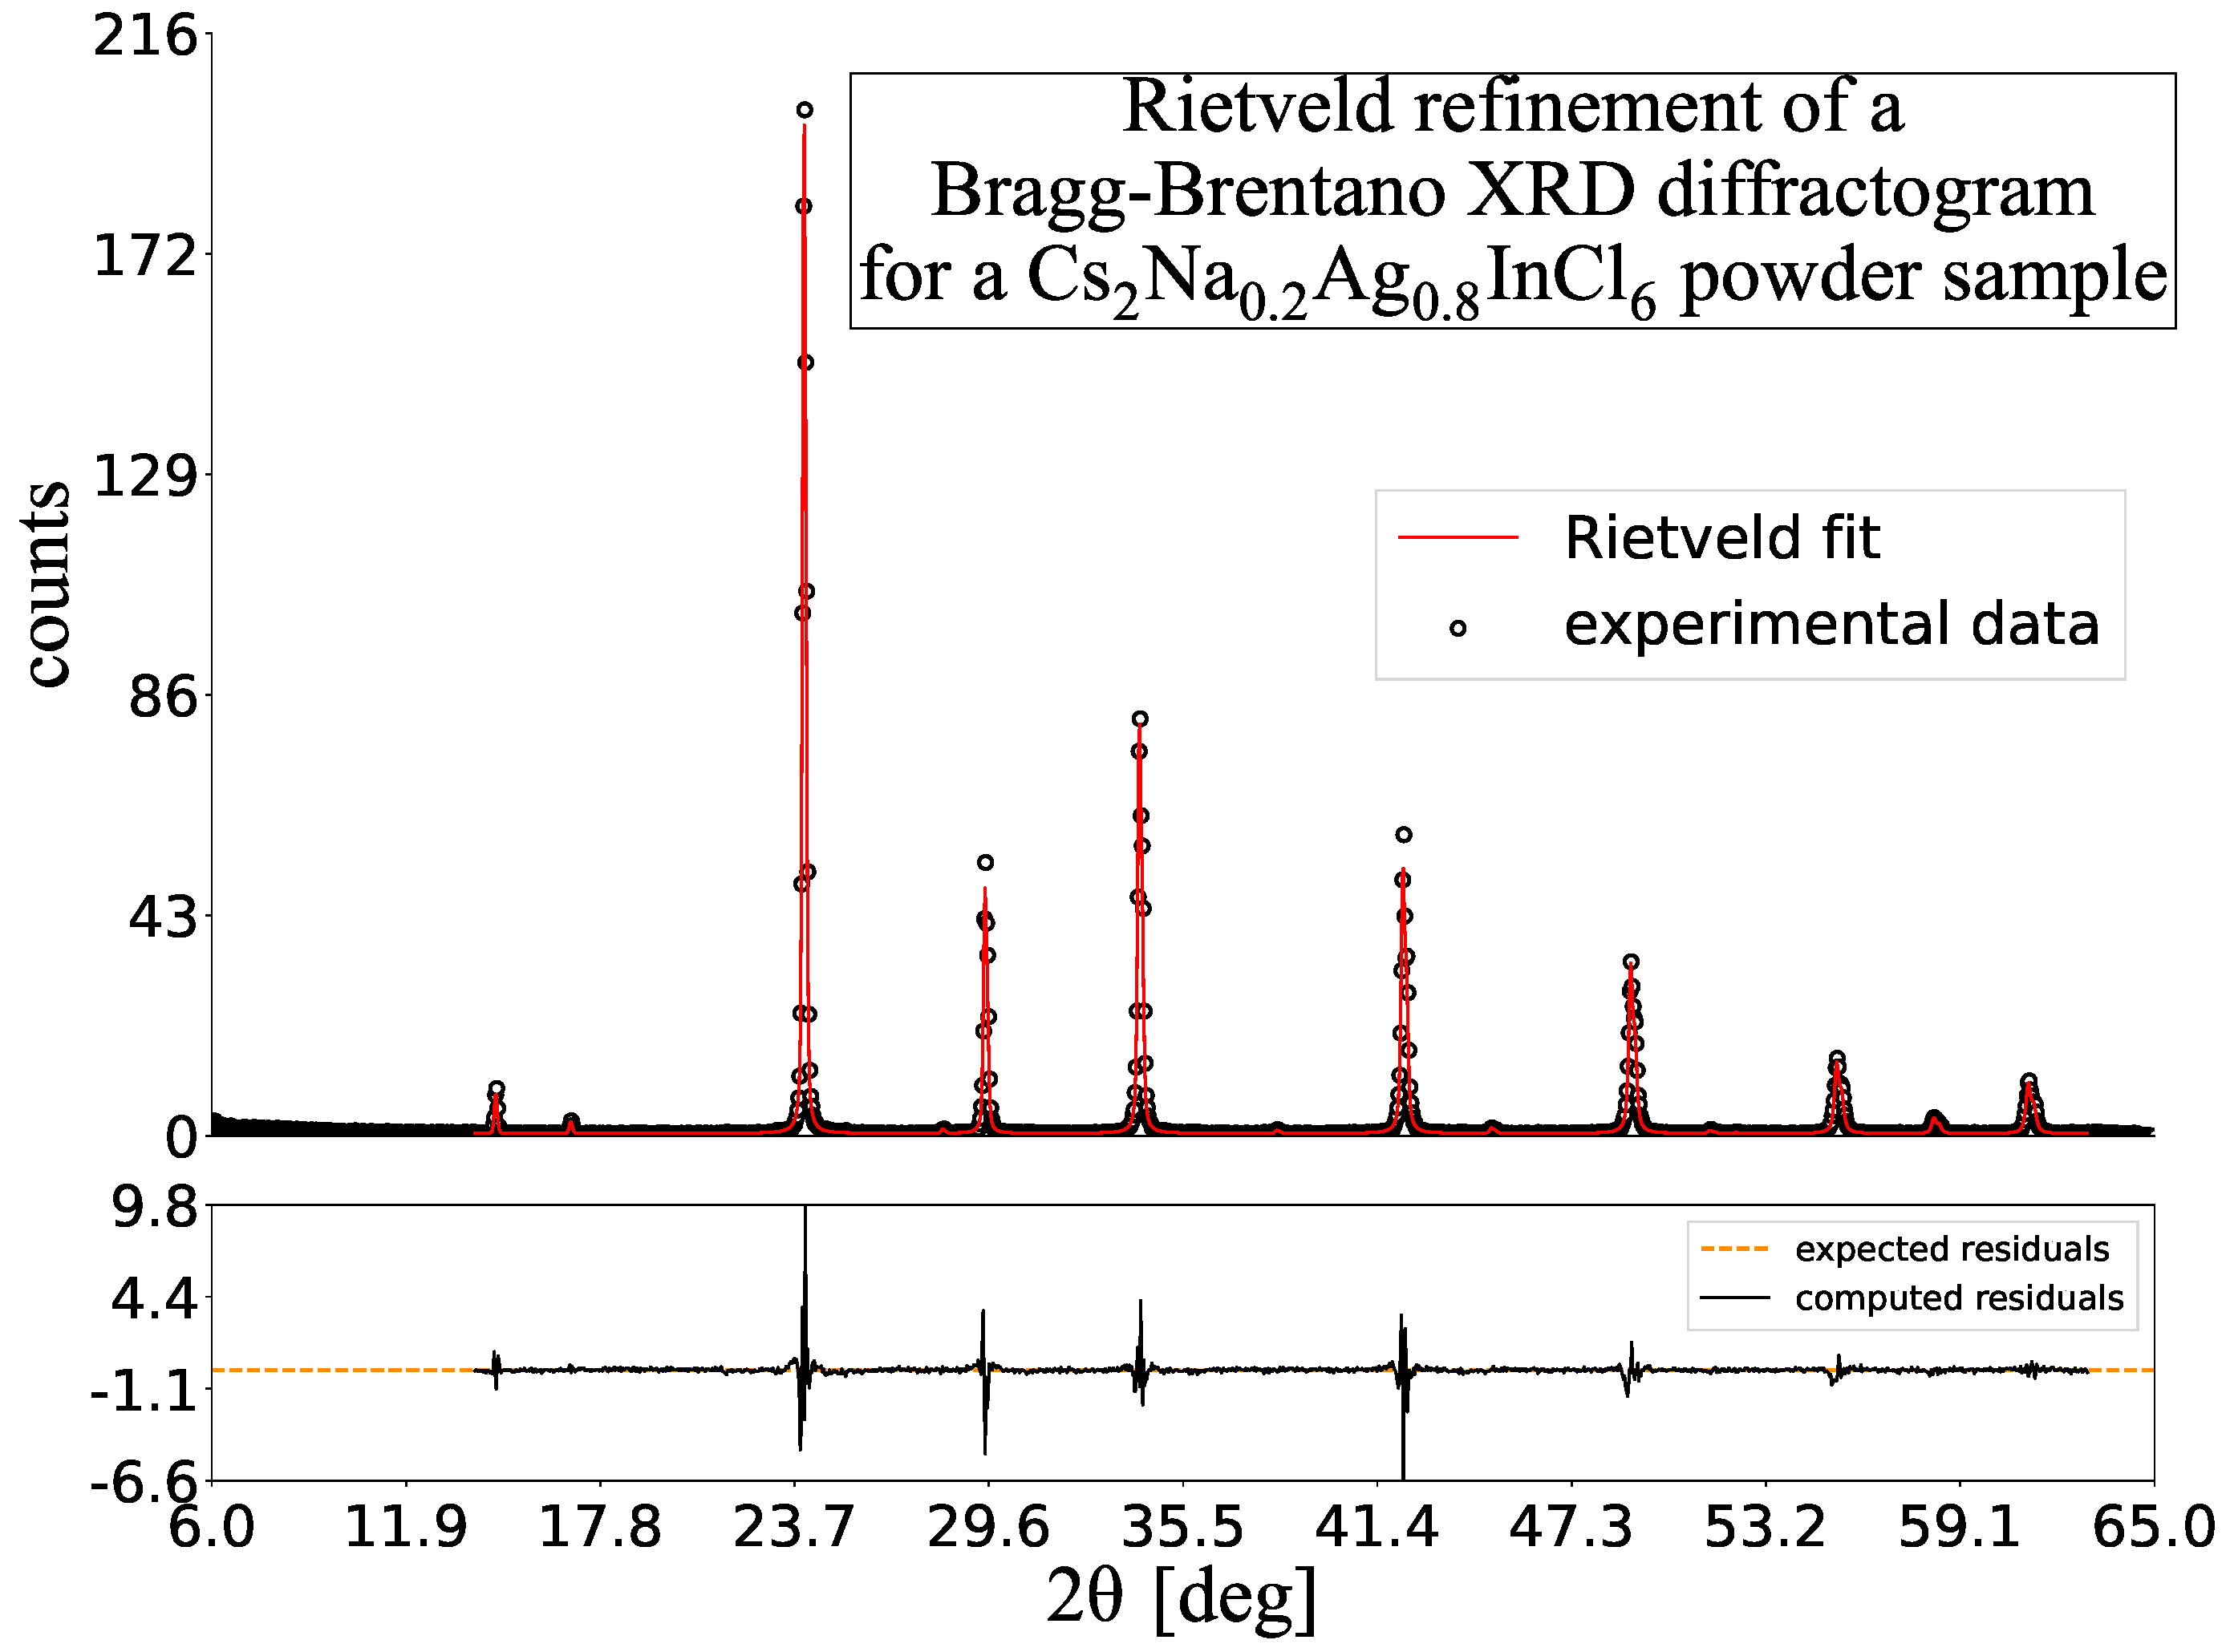
\includegraphics[width = 1\linewidth]{../Datasets/A02_Cs2Na0.2Ag0.8InCl6.pdf}
  \caption{Fit Rietveld per un diffrattogramma di Cs$_2$Ag$_{0.8}$Na$_{0.2}$InCl$_6$ in polvere.}
  \label{fig: Ag08Na02}
\end{figure}

\begin{figure}[htbp]
  \centering
  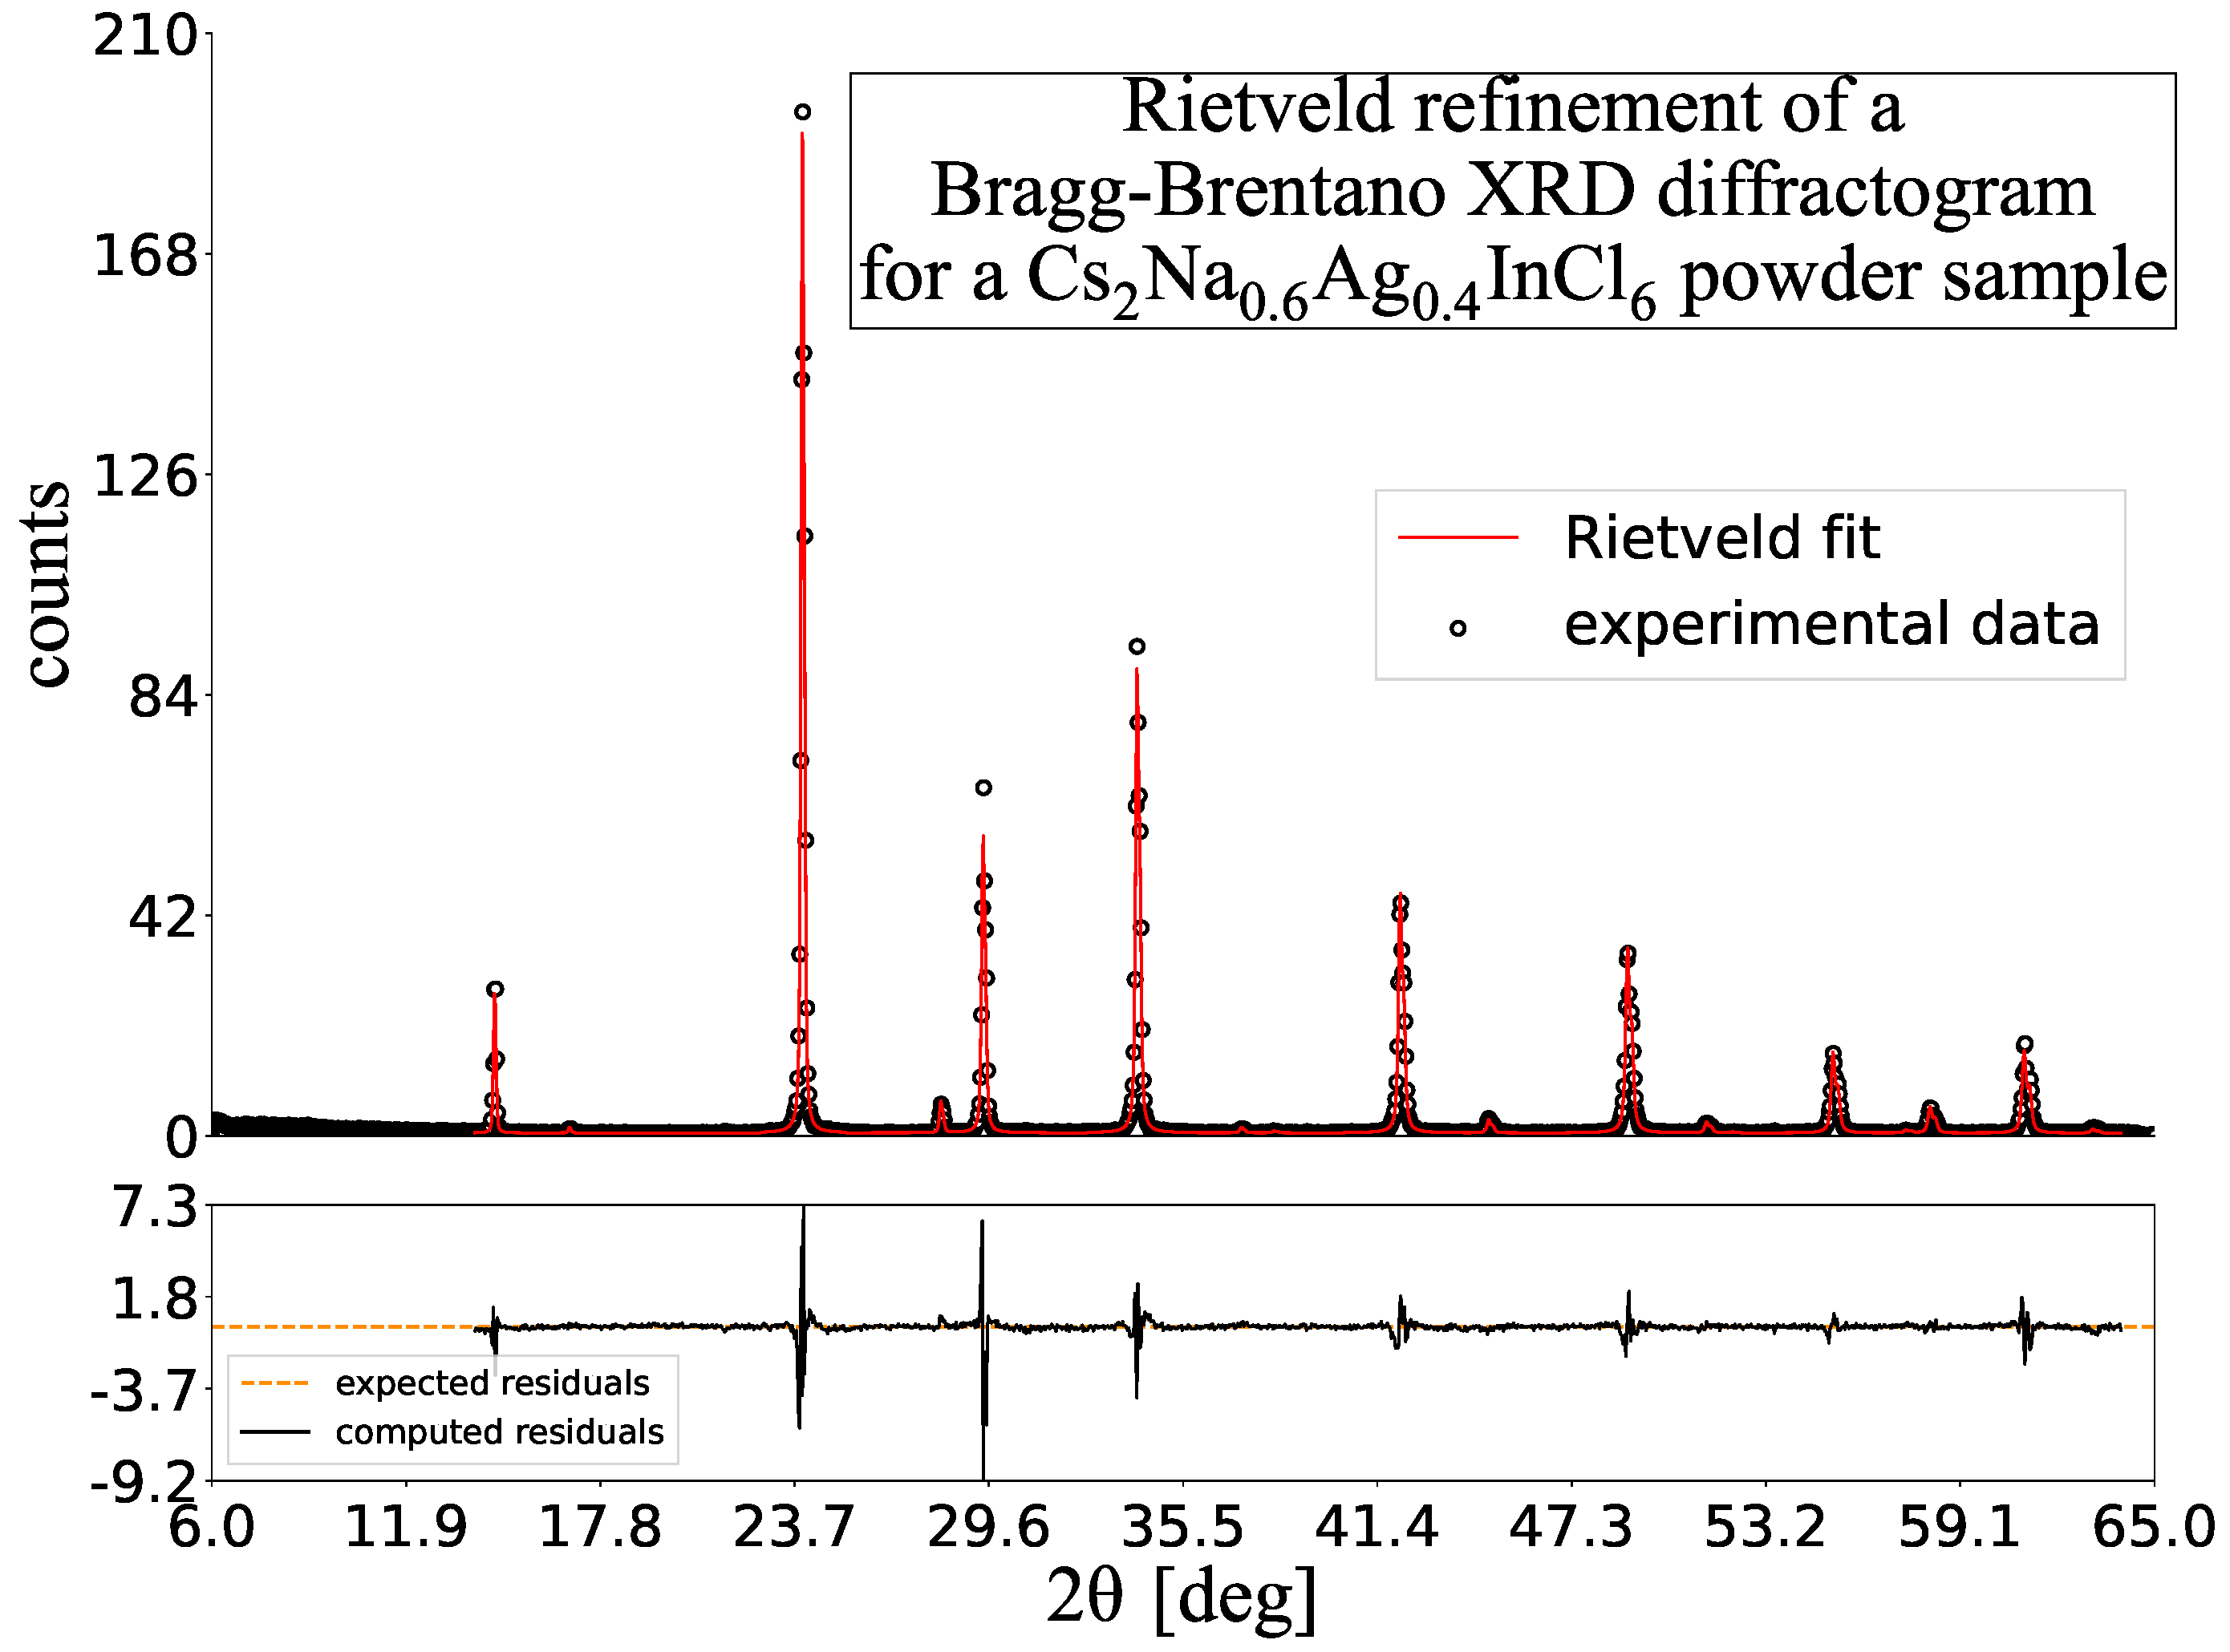
\includegraphics[width = 1\linewidth]{../Datasets/A04_Cs2Na0.6Ag0.4InCl6.pdf}
  \caption{Fit Rietveld per un diffrattogramma di Cs$_2$Ag$_{0.4}$Na$_{0.6}$InCl$_6$ in polvere.}
  \label{fig: Ag04Na06}
\end{figure}

Infine, è tempo di rilasciare il vincolo sulla quantità bersaglio del fit, ovvero la costante reticolare. A questo punto, secondo l'equazione \ref{eq: Rwp}, si è ottenuto un valore che si aggira attorno al $20\%$. A seguito di un'osservazione empirica di un grado di bontà della regressione non soddisfacente, si è scelto di raffinare anche gli elementi della matrice B, che appare nel termine del fattore di struttura del cristallo.

\begin{center}
\begin{table}[htbp]\setlength\belowcaptionskip{-20pt}
    \centering
\begin{tabular}{cc}
    \hline
    \textbf{campione} & $\mathbf{R_{wp}}$ ($\%$) \\
    \hline
    Cs$_2$AgInCl$_6$ & $9.75$\\
    Cs$_2$NaInCl$_6$ & $13.00$\\
    Cs$_2$Ag$_{0.8}$Na$_{0.2}$InCl$_6$ & $9.15$\\
    Cs$_2$Ag$_{0.4}$Na$_{0.6}$InCl$_6$ & $10.36$\\
    \hline
\end{tabular}
\caption{Valori-$R$ \emph{Weighted Pattern} di fit Rietveld, per i rispettivi diffrattogrammi.}
\label{tab: Rwp}
\end{table}
\end{center}

In tabella \ref{tab: Rwp} sono elencate le stime finali per i valori-$R$ \emph{Weighted Pattern} (come in tabella \ref{tab: delta2theta}, per completezza, sono stati compresi anche i campioni il cui fit non è stato ancora discusso). Salta all'occhio il risultato ottenuto per il campione Cs$_2$NaInCl$_6$, il cui maggiore valore, rispetto alle controparti, si attribuisce all'adattamento rozzo del file ".cif" per il campione Cs$_2$AgInCl$_6$.

Spostando l'attenzione alle figure \ref{fig: Ag08Na02} e \ref{fig: Ag04Na06}, come suggeriscono le tabelle \ref{tab: delta2theta} e \ref{tab: Rwp}, il raffinamento, per i campioni Cs$_2$Ag$_{0.8}$Na$_{0.2}$InCl$_6$ e Cs$_2$Ag$_{0.4}$Na$_{0.6}$InCl$_6$, ha subito un processo evolutivo simile a quello appena descritto. Infatti, a causa della composizione quaternaria di queste polveri, si è partiti dal file ".cif" per il campione Cs$_2$AgInCl$_6$ (considerato più affidabile della controparte Cs$_2$NaInCl$_6$) e si è aggiunto il quarto elemento, ovvero il sodio, modificando la concentrazione totale iniziale, sia di quest'ultimo sia dell'argento, in accordo con i valori nominali già noti delle rispettive concentrazioni parziali. Successivamente, si è rimosso il vincolo anche sulle percentuali di occupazione e si è lasciato che il software MAUD completasse il fit.
\begin{center}
\begin{table}[htbp]\setlength\belowcaptionskip{-20pt}
    \centering
\begin{tabular}{cc}
    \hline
    \textbf{campione} & $\mathbf{a}$ ($\text{\AA}$) \\
    \hline
    Cs$_2$AgInCl$_6$ & $10.4805 \pm 0.0002$ \\
    Cs$_2$NaInCl$_6$ & $10.4898 \pm 0.0002$\\
    Cs$_2$Ag$_{0.8}$Na$_{0.2}$InCl$_6$ & $10.5093 \pm 0.0005$\\
    Cs$_2$Ag$_{0.4}$Na$_{0.6}$InCl$_6$ & $10.5318 \pm 0.0003$\\
    \hline
\end{tabular}
\caption{Costanti reticolari $a$ calcolate secondo fit Rietveld, per i rispettivi diffrattogrammi.}
\label{tab: a}
\end{table}
\end{center}
La tabella \ref{tab: a} mostra i risultati ottenuti per ogni costante reticolare.

Esplicitando $x$ nell'equazione \ref{eq: Vegard}, è finalmente possibile stimare il valore di concentrazione relativa parziale tra i due elementi, argento e sodio, che condividono gli stessi siti di occupazione. Si è posto 
\begin{center}
\begin{table}[htbp]\setlength\belowcaptionskip{-20pt}
    \centering
\begin{tabular}{cc}
    \hline
    \textbf{campione} & $\mathbf{x}$\\
    \hline
    Cs$_2$Ag$_{0.8}$Na$_{0.2}$InCl$_6$ & $0.180 \pm 0.006$\\
    Cs$_2$Ag$_{0.4}$Na$_{0.6}$InCl$_6$ & $0.560 \pm 0.011$\\
    \hline
\end{tabular}
\caption{Concentrazioni relative parziali $x$ di argento e sodio, in perovskiti del tipo Cs$_2$Ag$_{1-x}$Na$_{x}$InCl$_6$, calcolate secondo la legge di Vegard.}
\label{tab: x}
\end{table}
\end{center}
La tabella \ref{tab: x} mostra le stime computate. L'errore sulla misura è determinato secondo propagazione per radice quadrata della somma in quadratura delle derivate parziali di ogni grandezza coinvolta.


\section*{Conclusioni}




\onecolumn
\newpage
\printbibliography

\newpage
\twocolumn
\section*{Appendice}


\end{document}